
\section{システムクロック校正}

端末のシステムクロックの進みかたはハードウェアごとに微妙に異なる.
そのため,同期してから長時間経つと,次第に端末間で遅延が生じる.
このことは,同一音源を同期的に再生し続けると,次第にずれが聞き取れるようになってくることを意味する.
この遅延を検出する手法について述べる.

端末 A のクロックを $S_A$,
端末 B のクロックを $S_B$ して,
時刻 $t$ 後に
A のサンプル数が $i$ ,
B のサンプル数が $i+d$ だけ異なっているとする(図\ref{fig:phaseshift2}).
このとき,Aを基準とした遅延比率 $S_B/S_A$ を求めたい.

\begin{figure}[tb]\centering
  \hspace{-2mm}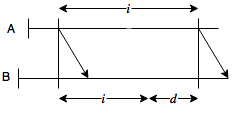
\includegraphics[clip,width=1.1\hsize]{img/phase_shift2.png}
  \caption{phaseshift2}\label{fig:phaseshift2}
\end{figure}

図より

$$\begin{aligned}
\frac{i}{S_A} &= \frac{i+d}{S_B} = t \\
\frac{S_B}{S_A} &= \frac{i+d}{i}
\end{aligned}$$

である.
遅延の検出においては,端末間の相対距離に変化がない限り,
端末Aが端末Bへとパルスを発生するだけで良く,
端末BはAへと返答パルスを返す必要はない.
既に同期済みでありAからBへの伝搬時間は算出済みだからである.



\section{音圧校正}
スマートデバイス毎にマイクロホンやスピーカのアンプ出力は異なるため,そのままではDBAP法は使えない.
ここでは,機器ごとの音圧を校正する手法を示す.

LTI(線形時不変)システムを仮定する.
$N$ 台の端末の番号を $i,j \in \{1\dots N\}$ とする.
端末 $i$ から端末 $j$ への信号伝達を考える.
$e$ を端末 $i$ で生成した単位振幅,
$v_i$ を端末 $i$ のスピーカアンプの増幅係数,
$m_j$ を端末 $j$ のマイクロホンアンプの増幅係数,
$d_{ij}=d_{ij}$ を $ij$ 間の測定距離,
$x_{ij}$ を $j$ が観測した $i$ からの信号の振幅とする.
音波の振幅は距離に反比例して減衰することが知られているので,
音声信号の伝達は

\begin{figure}[tb]\centering
  \hspace{-2mm}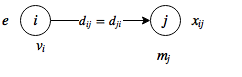
\includegraphics[clip,width=1.1\hsize]{img/sound_pressure_calibration.png}
  \caption{soundpressurecalibration}\label{fig:soundpressurecalibration}
\end{figure}

$$
e v_i \frac{1}{d_{ij}} m_j = x_{ij}
$$

とモデル化できる(図\ref{fig:soundpressurecalibration}).
このとき,ある端末 $k$ の出力係数 $v_k$ と他の端末 $i$ の出力係数 $v_i$ との比 $v_i/v_k$ を求めたい.

$$
e v_i m_j = x_{ij}d_{ij}
$$

なので

$$\begin{aligned}
\frac{e v_j m_j}{e v_k m_j} &= \frac{x_{ij} d_{ij}}{x_{kj} d_{kj}} \\
\frac{v_j}{v_k} &= \frac{x_{ij} d_{ij}}{x_{kj}d_{kj}} \\
\end{aligned}$$

である.
観測した振幅 $x_{ij}$ および測定距離 $d_{ij}$ は誤差を含むので,
それらを平均した $\hat{v_i}$ は

$$
\frac{\hat{v_i}}{v_k} = \frac{1}{N} \sum_{i\neq j \neq k} \frac{x_{ij} d_{kj}}{x_{kj}d_{ij}} \\
$$

と定義できる.$d_{ii}$ のときは距離が0となりゼロ除算が発生するので,
$i\neq j \neq k$ としている.

一番出力の低い端末 $k$ の出力係数 $v_k$ を基準とすることで,
すべての端末において定格出力を守ることができる.

\section{隣接ノードでない端末間の同期,音圧校正,クロック校正}


互いに互いの信号を検出できなかったノード間での校正を考える.
図\ref{fig:networktopology}に隣接ノードではない端末を含むネットワークを示す.

\begin{figure}[tb]\centering
  \hspace{-2mm}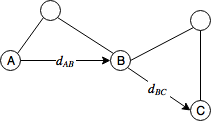
\includegraphics[clip,width=1.1\hsize]{img/network_topology.png}
  \caption{networktopology}\label{fig:networktopology}
\end{figure}

このとき端末 A と端末 C 間では同期・測距ができていないが,
互いに端末 B とは同期・測距できているという状況である.

\subsection{同期}

時刻の基準となる
端末 $A$ がパルスを発した時間を $t_{AA}$ として
そのパルスが端末 $B$ に届いた時間は $t_{AB}$ とする.
また,
端末 $B$ がパルスを発した時間を $t_{AB}$ として
そのパルスが端末 $C$ に届いた時間は $t_{BC}$ とする.
そしてそれぞれの伝達時間を $d$ とすると図\ref{fig:reldelay}のようになる.

\begin{figure}[tb]\centering
  \hspace{-2mm}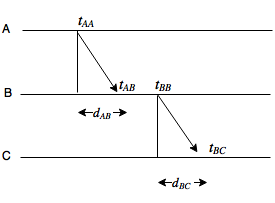
\includegraphics[clip,width=1.1\hsize]{img/rel_delay.png}
  \caption{reldelay}\label{fig:reldelay}
\end{figure}

このとき,まず端末 $C$ は端末 $B$ と同期して,
その後端末 $B$ と端末 $A$ の時刻ずれ情報をもとにさらに端末 $A$ との同期ができる.


\subsection{音圧校正}

端末 $A$ を基準に音圧校正を考えると

$$
\frac{v_B}{v_A} = \frac{x_{iB} d_{iB}}{x_{AB}d_{AB}} \\
\frac{v_C}{v_B} = \frac{x_{iC} d_{iC}}{x_{BC}d_{BC}} \\
$$

であるので

$$
\frac{v_C}{v_A} =
\frac{v_B v_C}{v_A v_B} =
\frac{x_{iB} x_{iC} d_{iB} d_{iC}}{x_{AB} x_{BC} d_{AB} d_{BC}}
$$

とすれば端末 A と端末 C の出力比率を求められる.

\subsection{クロック校正}
